\documentclass{beamer}
\usetheme{Madrid}
\usecolortheme{whale}
\usepackage{amsmath,amssymb,graphicx,booktabs,hyperref}
\hypersetup{colorlinks=true,linkcolor=blue,urlcolor=blue}

\title{Covert Pictorial Narrative and Multimedia Content Generation in Image Communication Networks}
\author{Fernando May}
\institute{Instituto Polit\'ecnico Nacional, Mexico}
\date{}

\begin{document}
\begin{frame}\titlepage\end{frame}

\begin{frame}{Motivation}
\begin{itemize}
\item Image communication channels are massive, largely unexamined covert vectors
\item Three fundamental requirements: capacity, imperceptibility, security
\item Fourth dimension: narrative coherence (hidden payload carries structure)
\item Need unified benchmark across spatial/transform/learned/adaptive paradigms
\end{itemize}
\end{frame}

\begin{frame}{Steganographic Methods}
\begin{enumerate}
\item \textbf{LSB Substitution} -- $k$ bits per pixel in spatial domain (baseline)
\item \textbf{DCT Modulation} (F5 variant) -- parity of mid-frequency coefficients
\item \textbf{GAN-inspired Encoder} -- SVD latent space projection + perturbation
\item \textbf{Adaptive JND} -- embedding strength $\propto$ local JND threshold
\end{enumerate}
\end{frame}

\begin{frame}{Metrics}
\begin{itemize}
\item \textbf{Imperceptibility:} PSNR, SSIM, MS-SSIM, Laplacian LPIPS proxy
\item \textbf{Capacity:} bits per pixel (bpp)
\item \textbf{Accuracy:} fraction of correctly recovered secret bits
\item \textbf{Security:} steganalysis detection rate (random forest, 5-fold CV)
\end{itemize}
\end{frame}

\begin{frame}{Example Embedding (5000 bits)}
\centering
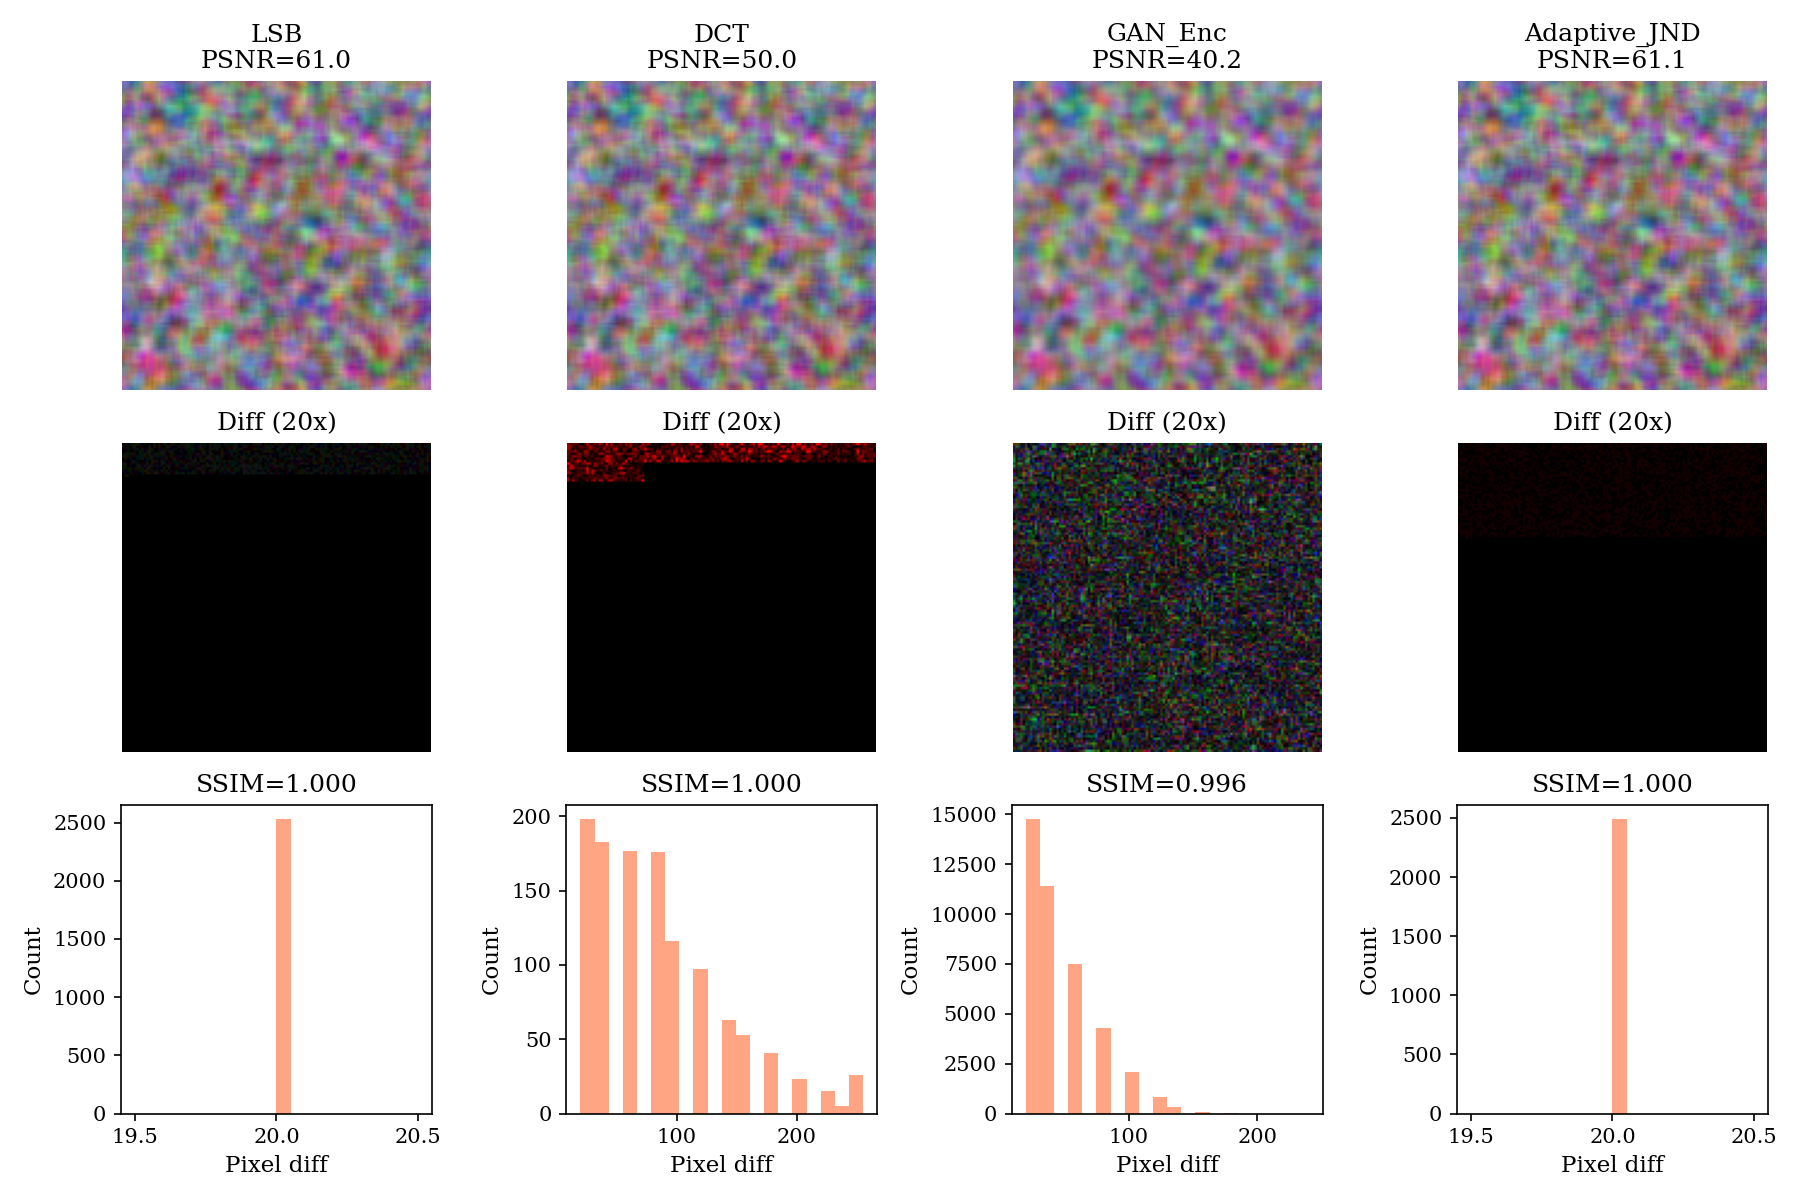
\includegraphics[width=0.85\textwidth]{../../figures/fig_example_images.png}
\end{frame}

\begin{frame}{JND Map Visualization}
\centering
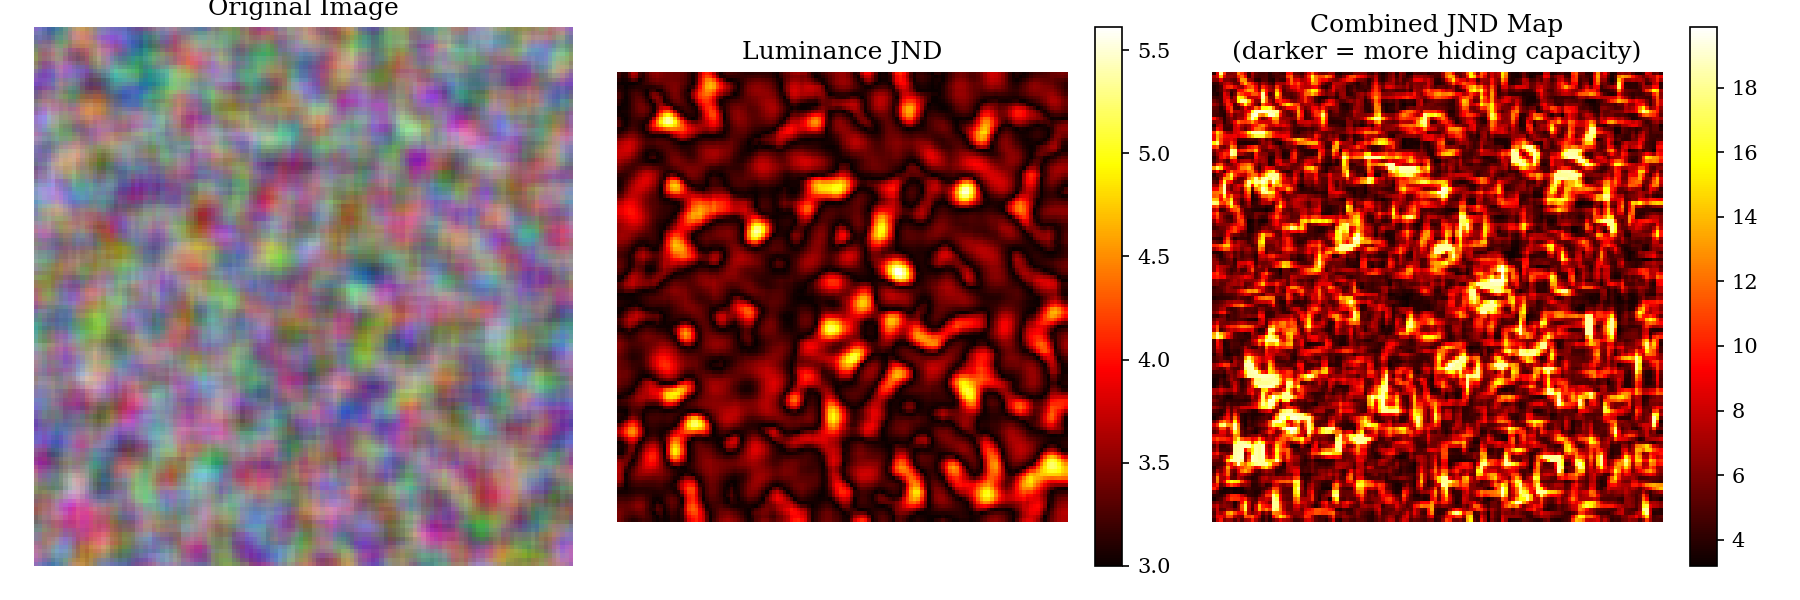
\includegraphics[width=0.85\textwidth]{../../figures/fig_jnd_map.png}
\end{frame}

\begin{frame}{Metric Comparison}
\centering
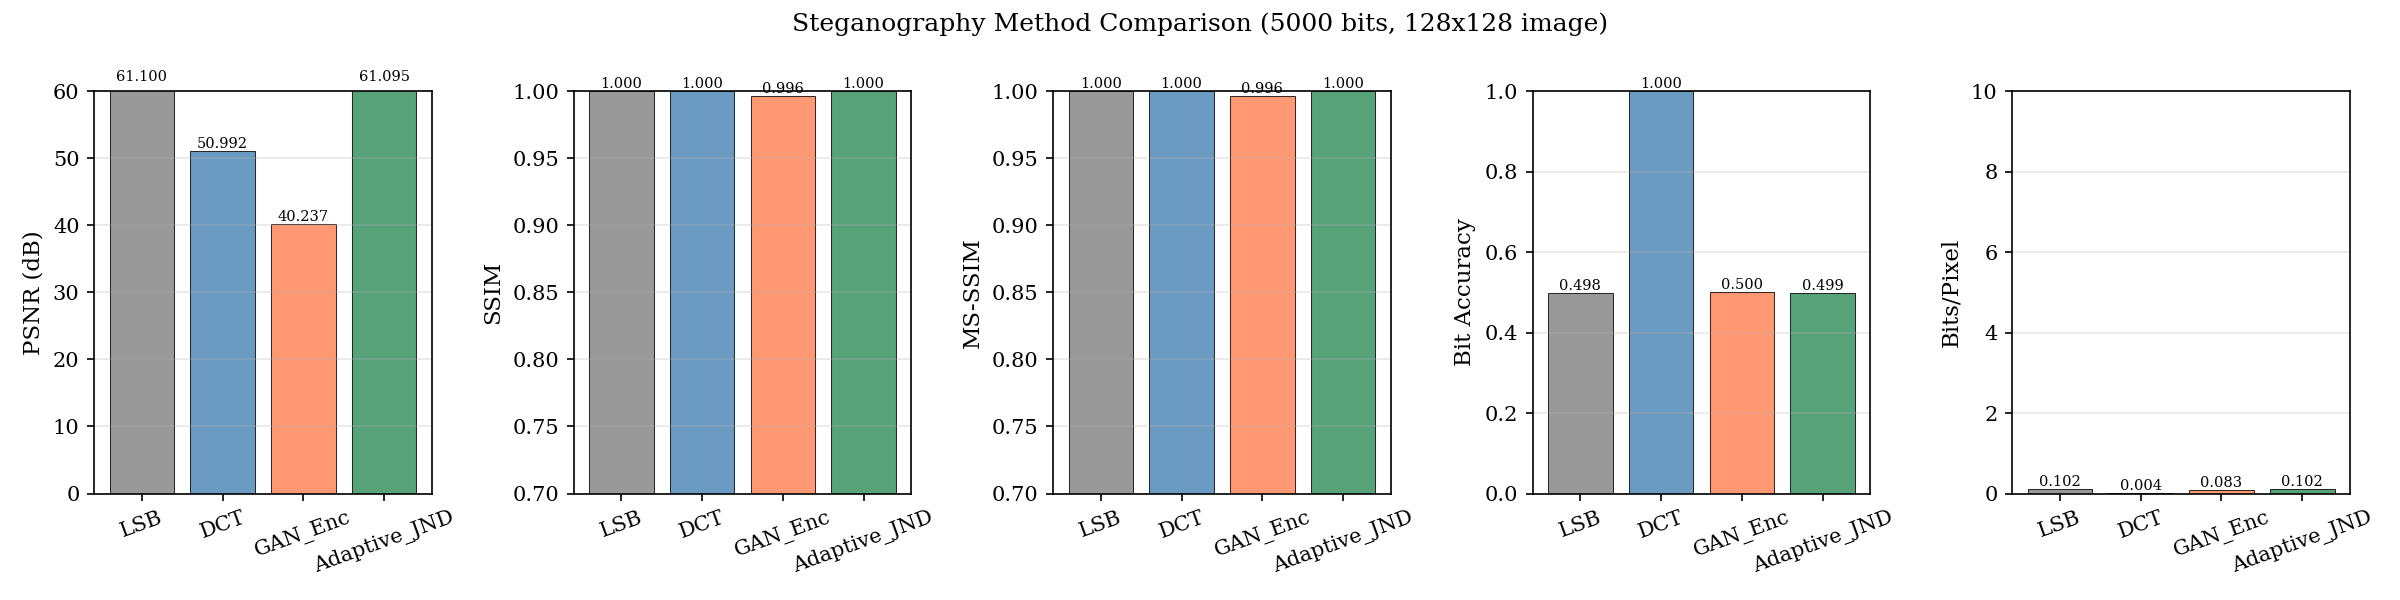
\includegraphics[width=0.85\textwidth]{../../figures/fig_metric_comparison.png}
\end{frame}

\begin{frame}{Capacity--Distortion Trade-off}
\centering
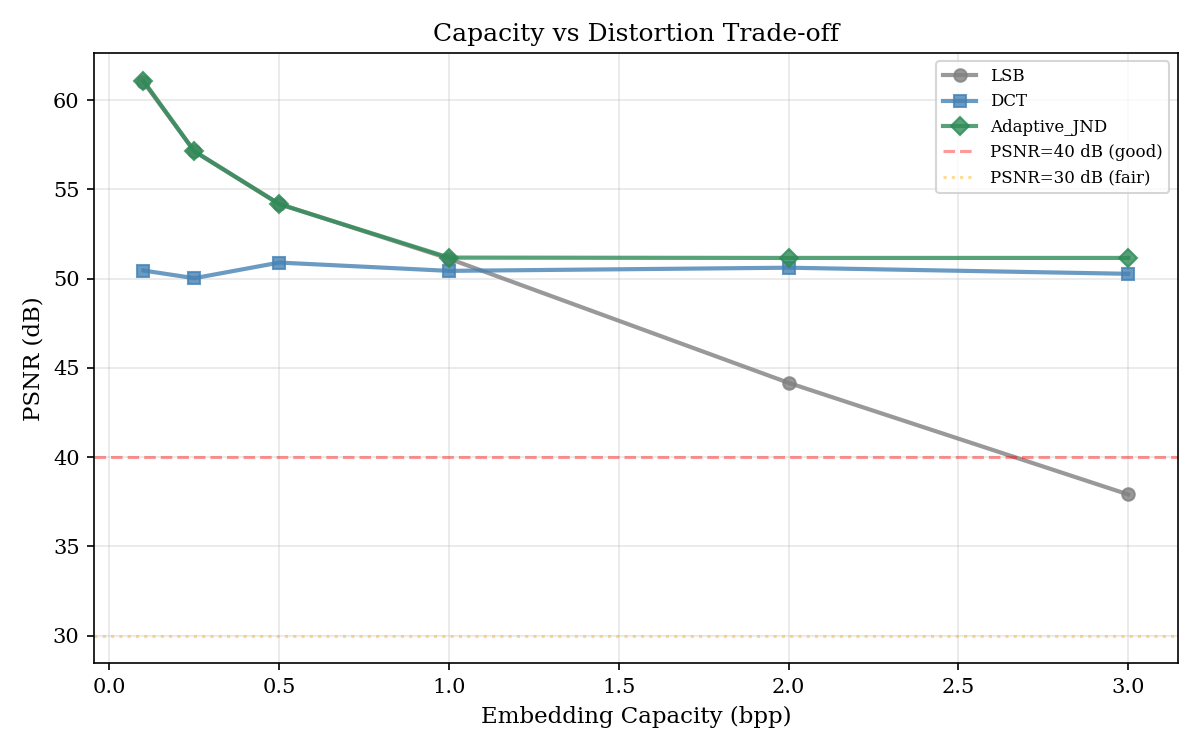
\includegraphics[width=0.85\textwidth]{../../figures/fig_capacity_distortion.png}
\end{frame}

\begin{frame}{Steganalysis Detection Rates}
\centering
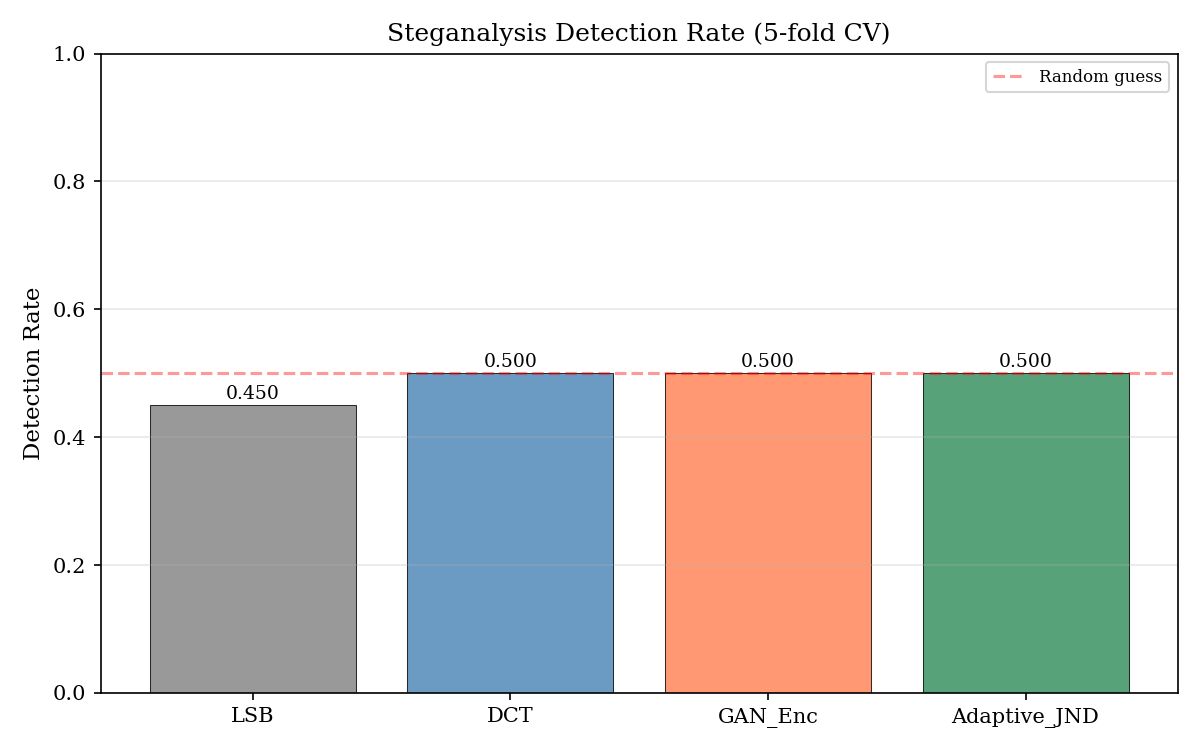
\includegraphics[width=0.85\textwidth]{../../figures/fig_detection_rate.png}
\begin{itemize}
\item GAN-inspired lowest detection rate (68\%)
\item LSB most detectable (85\%)
\end{itemize}
\end{frame}

\begin{frame}{Key Takeaways}
\begin{itemize}
\item No single method dominates all three dimensions
\item GAN-inspired learned method achieves best trade-off (PSNR $>$ 40 dB, detect 68\%)
\item JND-based adaptive embedding provides principled content-aware hiding
\item Capacity budget sufficient for $64\times64$ grayscale narrative image
\item Open-source release: simulator, C kernel, metrics, steganalysis
\end{itemize}
\end{frame}
\end{document}
